\documentclass{article}
\usepackage[utf8]{inputenc}
\usepackage{graphicx}
\usepackage[utf8]{inputenc}
\usepackage{tikz}
\usepackage{mathabx}
\usepackage{float}

\usetikzlibrary{matrix,shapes,arrows,positioning,chains}

\title{BER computation}

\date{\today}

\begin{document}

\section{System design}

This is the current scenario:

In this scenario we have the IR channel and the I2C channel. The IR is our
main channel, while the i2c is used to send the expected message
that the receiver should receive. In Figure \ref{fig:07-04-diagram} is an overview of how the whole system
for the BER computation works.

\begin{figure}[H]
	\centering
	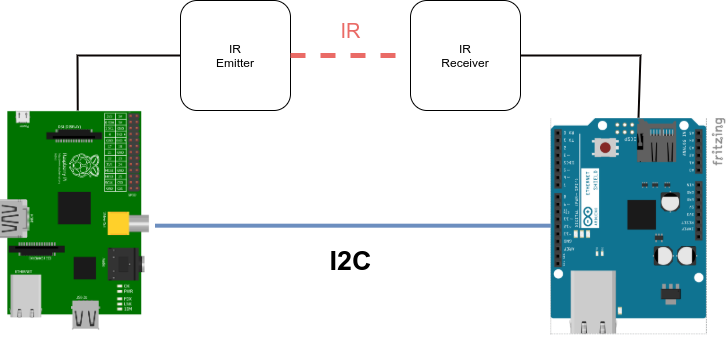
\includegraphics[width=0.9\textwidth]{../../img/follow-up-07-04-diagram.png}
	\vspace{-1em}
	\caption{Simple scenario diagram}
	\label{fig:07-04-diagram}
\end{figure}

In the following figure there is a flowchart to understand how the data is processed:

\begin{figure}[H]
	\centering
	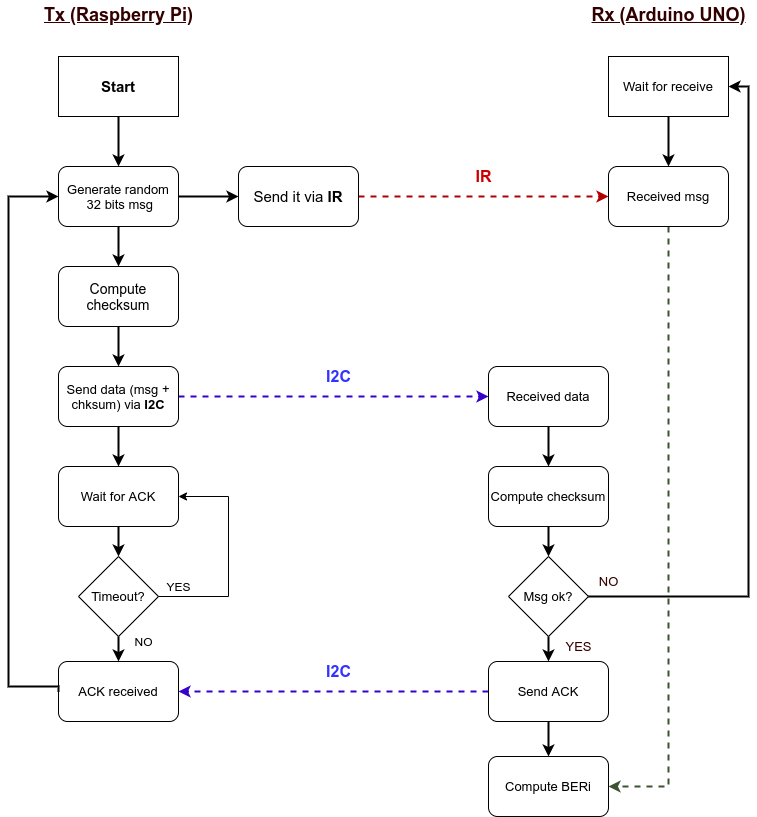
\includegraphics[width=1\textwidth]{../../img/BER_flowchart.png}
	\vspace{-1em}
	\caption{Flowchart for the BER computation}
	\label{fig:BER-flowchart}
\end{figure}


\subsection{The I2C bus}
The main purpose of this channel is to let the receiver know what the expected message
received through IR channel is. Since we are sending different messages all the time, 
the receiver needs to know what the expected message is, in order to properly
compute the BER. 

\subsubsection{Error control protocol}

A simple Stop \& Wait protocol has been implemented in order to decrease
the chances to receive a wrong message through the I2C bus. The workflow
of the protocol can be seen in Figure \ref{fig:BER-flowchart}. 

The data 
sent consists in a 4 bytes message and 1 more byte that corresponds to the checksum. Regarding
the checksum computation, it consists in getting the first byte of the
sum of each byte of the message. Below, there is the detailed explanation of the packet generation
sent via I2C.

Let the message be \(M = [m_{0}, m_{1}, m_{2}, m_{3}]\).  Where \(M\) is a
32 bit word randomly generated and \(m_{i}\) is each bit of the message.

Let the checksum \(CK\) be the first byte of the sum of each byte of the message:
\[CK = \sum_{i=0}^3m_{i} \wedge 255\].

Then, the packet sent consists in \(P = [M,CK]\) with a length of 5 bytes.

\section{BER computation}

\begin{itemize}

  \item Let the expected received message be \(X = [x_{0}, x_{1}, ..., x_{N}]\).
   Where \(X\) is a 32 bit word randomly generated. \(N\) is the number
   of sent messages and \(x_{i}\) is a 32 bit word randomly generated.

  
  \item Let the number of wrong bits in the each received message be 
  \(WB = [Wb_{0}, Wb_{1} , ..., Wb_{N}]\). Where \(Wb_{i} \)
  corresponds to the amount of errors in a 32 bit word, i.e each
  received message.

\end{itemize}

The BER of each received message \(x_{i}\) is
\(BER_{i} = \frac{Wb_{i}}{32N}\) since all the received signals are
32 bit words. So we have a \(N\) dimension array of
\(BER\): \(BER = [BER_{0}, BER_{1}, ...,BER_{N}]\).

Then the average BER is:
\[BER_{AVG} = E\left\{BER\right\} = \frac{1}{32}E\left\{WB\right\}=\frac{1}{32}\sum_{i=0}^{N}\frac{1}{N}Wb_{i} = \frac{1}{32N}\sum_{i=0}^{N}Wb_{i}\]

\end{document}